\documentclass[border=4pt]{standalone}
\usepackage{tikz}
\usepackage{amsmath}
% Shared TikZ style: validated categorical palette (FP32 blue, FP16 orange, INT8 green, FP8 amber), light print surface.
\usetikzlibrary{arrows.meta,positioning,fit,backgrounds,calc,shapes.geometric}
\definecolor{fp32}{HTML}{2A78D6}
\definecolor{fp16}{HTML}{EB6834}
\definecolor{int8}{HTML}{1BAF7A}
\definecolor{fp8}{HTML}{EDA100}
\definecolor{ink}{HTML}{0B0B0B}
\definecolor{ink2}{HTML}{52514E}
\definecolor{muted}{HTML}{898781}
\definecolor{grid}{HTML}{E1E0D9}
\definecolor{surface}{HTML}{FCFCFB}
\definecolor{wash}{HTML}{F0EFEC}
\tikzset{
  font=\sffamily\small,
  box/.style={draw=muted, rounded corners=3pt, fill=surface, align=center, inner sep=4pt, text=ink},
  stage/.style={box, minimum height=1.0cm, text width=2.6cm},
  data/.style={box, fill=wash, draw=grid},
  result/.style={box, text width=2.9cm, minimum height=1.35cm},
  arrow/.style={-{Stealth[length=2.2mm]}, draw=ink2, line width=0.7pt},
  feedback/.style={arrow, dashed, draw=int8},
  tag/.style={font=\sffamily\scriptsize, text=ink2},
  group/.style={draw=grid, rounded corners=5pt, inner sep=6pt, line width=0.8pt},
}

\begin{document}
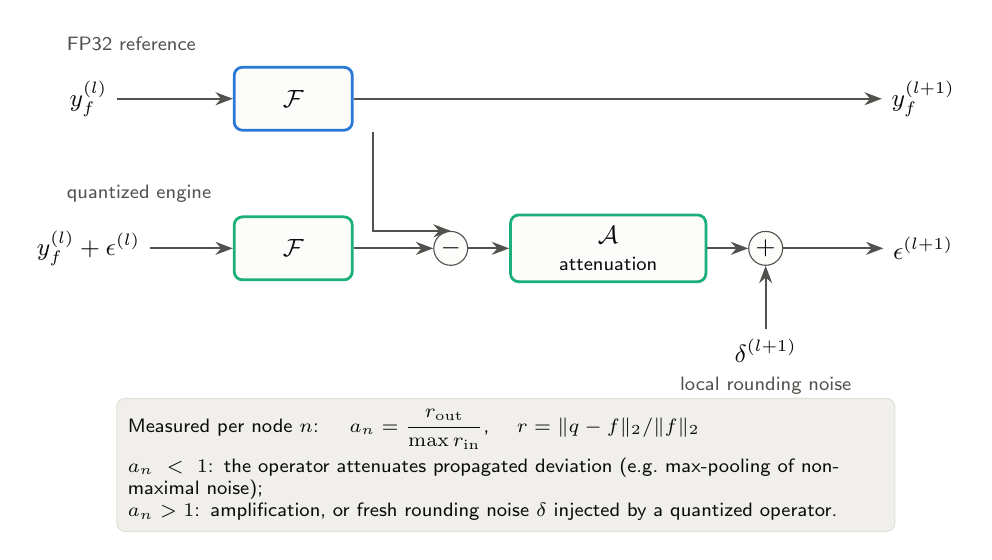
\begin{tikzpicture}[
  op/.style={box, minimum width=1.5cm, minimum height=0.8cm},
  sum/.style={circle, draw=ink2, fill=surface, inner sep=1pt, font=\small},
  sig/.style={font=\small, text=ink}]
% FP32 path
\node[sig] (yf) at (0,1.3) {$y_f^{(l)}$};
\node[op, draw=fp32, line width=1pt] (Ff) at (2.6,1.3) {$\mathcal{F}$};
\node[sig] (yf1) at (10.6,1.3) {$y_f^{(l+1)}$};
\draw[arrow] (yf) -- (Ff); \draw[arrow] (Ff) -- (yf1);
\node[tag, anchor=west] at (-0.4,2.0) {FP32 reference};
% quantized path
\node[sig] (yq) at (0,-0.6) {$y_f^{(l)}+\epsilon^{(l)}$};
\node[op, draw=int8, line width=1pt] (Fq) at (2.6,-0.6) {$\mathcal{F}$};
\node[sum] (minus) at (4.6,-0.6) {$-$};
\node[op, draw=int8, line width=1pt, text width=2.2cm] (A) at (6.6,-0.6) {$\mathcal{A}$\\[-1pt]\scriptsize attenuation};
\node[sum] (plus) at (8.6,-0.6) {$+$};
\node[sig] (e1) at (10.6,-0.6) {$\epsilon^{(l+1)}$};
\node[sig] (d) at (8.6,-1.9) {$\delta^{(l+1)}$};
\node[tag] at (8.6,-2.35) {local rounding noise};
\draw[arrow] (yq) -- (Fq); \draw[arrow] (Fq) -- (minus); \draw[arrow] (minus) -- (A);
\draw[arrow] (A) -- (plus); \draw[arrow] (plus) -- (e1); \draw[arrow] (d) -- (plus);
\draw[arrow] (Ff.south east) ++(0.25,0) |- (minus.north) ;
\node[tag, anchor=west] at (-0.4,0.1) {quantized engine};
% measured quantity
\node[box, fill=wash, draw=grid, text width=9.6cm, align=left, font=\sffamily\scriptsize] at (5.3,-3.35) {
Measured per node $n$: \quad $a_n=\dfrac{r_\mathrm{out}}{\max r_\mathrm{in}}$, \quad $r=\lVert q-f\rVert_2/\lVert f\rVert_2$\\[2pt]
$a_n<1$: the operator attenuates propagated deviation (e.g.\ max-pooling of non-maximal noise);\\
$a_n>1$: amplification, or fresh rounding noise $\delta$ injected by a quantized operator.};
\end{tikzpicture}
\end{document}
